\documentclass[a4paper, 12pt, garamond]{book}
\usepackage{cours-preambule}

\makeatletter
\renewcommand{\@chapapp}{Fiches -- numéro}
\makeatother

\begin{document}
\setcounter{chapter}{3}

\chapter{Régression linéaire}

\section{Principe}

La pratique de la science passe par deux pivots inséparables~: la
\textit{théorie} et la \textit{mesure}. La première pose un cadre de travail
pour aboutir à des conclusions sur le fonctionnement du monde physique sous la
forme de relations mathématiques, et la seconde relève des valeurs
expérimentales du monde physique pour en archiver les propriétés effectives.

L'une et l'autre se nourrissent conjointement~: une théorie physique pose une
loi et la mesure permet de la tester, ou un relevé expérimental particulier
permet de mettre en évidence un point sombre des cadres théoriques actuels. Il
reste que les sciences physiques ont pour unique objectif de rendre compte du
réel~; ainsi, si l'expérience est bien contrôlée, \textbf{c'est toujours la
	mesure qui clôt la discussion}.

Dans ce cadre, il est commun de disposer de deux jeux de données réelles
représentant des \textbf{grandeurs reliées} entre elles par une
loi physique (disons $x$ et $y$), et normalement compatibles avec une
\textbf{relation linéaire} mathématique~:
\[
	\boxed{y = ax+b}
\]
avec $a$ et $b$ des coefficients propres à la relation~:
\begin{itemize}
	\item $a$ le \textit{coefficient directeur}~;
	\item $b$ l'\textit{ordonnée à l'origine}.
\end{itemize}

La régression linéaire\ftn{Il faudrait en toute rigueur parler de régression
\textit{affine} et non linéaire.} vise à \textbf{tester l'accord entre mesure et
théorie}, et le cas échéant à \textbf{estimer les coefficients} et leurs
incertitudes. Elle repose sur la détermination de la meilleure droite qui serait
susceptible de représenter le nuage de points donné en deux dimensions par $x$
et $y$, en l'occurrence en minimisant la somme des distances au carré entre
chacun des points et la droite. Cet \textbf{écart aux points mesurés} est
caractérisé par un coefficient de corrélation, noté $r$, ou de régression, noté
$r^{2}$, et compris entre 0 (nul) et 1 (parfait).

\begin{tcb}(defi){Régression linéaire}
	Une régression linéaire est une \textbf{opération mathématique} entre des
	points de mesure $x_i$ et $y_i$ qui consiste à trouver les meilleurs
	coefficients $a$ et $b$ tels que $ax_i+b$ soient les plus proches en moyenne
	des points de mesures $y_i$.
\end{tcb}

Cette régression peut être faite à la main, mais la détermination des
coefficients ne sera pas rigoureuse. Nous allons ici détailler le processus pour
une régression \textit{via} un logiciel.

\section{Réalisation logicielle}
% Elle peut s'effectuer avec un logiciel sur ordinateur (\texttt{Latis Pro},
% \texttt{Regressi}…), avec un langage de programmation (\texttt{Python}…) ou
% directement à la calculatrice.

\subsection{À la calculatrice}

\begin{tcb}[breakable](expe)<itc>{TI 83+}
	\begin{itemize}[leftmargin=10pt]
		\item Appuyer sur \texttt{stats}.
		\item Dans le menu \texttt{EDIT} choisir \texttt{1~: Editer}.
		\item Entrer les deux séries de données~: l'abscisse dans la première colonne
		      \texttt{L1}, et l'ordonnée dans la seconde colonne \texttt{L2}.
		\item Dans le menu \texttt{graph stats}, choisir la première ligne.
		\item Choisir \texttt{Aff} pour afficher, puis le premier type, la liste
		      \texttt{L1} pour \texttt{ListeX} et la liste \texttt{L2} pour
		      \texttt{ListeY}.
		\item Appuyer sur \texttt{graphe} pour afficher le nuage de points.
		\item Pour déterminer les coefficients $a$, $b$ et $r$ ou $r^{2}$,
		      retourner dans \texttt{stats} puis aller dans le menu \texttt{CALC} et
		      choisir \texttt{4~: RegLin(ax+b)}. Appuyer sur \texttt{ENTER}.
	\end{itemize}
	\begin{isd}(expe)
		\tcbsubtitle{\fatbox{$r$ non indiqué}}
		\begin{itemize}[leftmargin=10pt]
			\item Appuyer sur \texttt{2nde} puis \texttt{catalog}.
			\item Choisir \texttt{Diagnostic On} ou \texttt{corelAff} selon la langue,
			      appuyer deux fois sur \texttt{ENTER}.
		\end{itemize}
		\tcblower
		\tcbsubtitle{\fatbox{Tracer la courbe}}
		\begin{itemize}[leftmargin=10pt]
			\item Aller dans \texttt{f(x)}, appuyer sur \texttt{var}.
			\item Choisir \texttt{5~: Statistiques}.
			\item Dans le menu \texttt{EQ} choisir \texttt{1}, puis \texttt{ENTER}.
			\item Aller dans \texttt{graphe} pour voir la droite.
		\end{itemize}
	\end{isd}
\end{tcb}

\begin{tcb}[breakable](expe)<itc>{Casio 35+}
	\begin{itemize}[leftmargin=10pt]
		\item Aller dans le mode \texttt{STAT}.
		\item Entre les deux séries de données dans \texttt{List1} et
		      \texttt{List2}.
		\item Appuyer sur \texttt{GRAPH} puis \texttt{SET}.
		\item Choisir le type de graphique \texttt{GraphType~: Scatter}. Mettre
		      \texttt{List1} dans \texttt{XList} pour l'abscisse et \texttt{List2}
		      dans \texttt{YList} pour l'ordonnée.
		\item Appuyer sur \texttt{ENTER}, et appuyer sur \texttt{GRAPH 1} pour
		      visualiser le nuage de points.
		\item Appuyer sur \texttt{CALC} puis \texttt{X} puis sur \texttt{ax+b} pour
		      obtenir une régression linéaire $y = ax+b$.
		\item Une fenêtre \texttt{LinearReg} affiche la pente $a$, l'ordonnée à
		      l'origine $b$ et le coefficient de corrélation $r^{2}$.
		\item Pour visualiser la droite, choisir \texttt{DRAW} en bas à droite.
	\end{itemize}
\end{tcb}

\begin{tcb}*(expe)<itc>"wip"{Numworks}
	Travail en cours…
	\vfill
\end{tcb}

\begin{tcb}[cnt, bld](impo){Attention~!}
	Il est plus que courant d'inverser les deux listes~!
\end{tcb}

\subsection{En \texttt{Python}}
\begin{python}
# =========================================================================== #
#                                   Imports                                   #
# =========================================================================== #

import numpy as np               # pour les tableaux et la gestion des données
import matplotlib.pyplot as plt  # pour les graphiques, l'affichage des données

# =========================================================================== #
#                            Données expérimentales                           #
# =========================================================================== #

X = np.array([0, 2, 4, 6, 8, 10])            # À modifier
Y = np.array([0.5, 7.9, 11, 17.5, 26, 31.8]) # À modifier

# =========================================================================== #
#                                  Régression                                 #
# =========================================================================== #

# Donne a le coefficient directeur et b l'ordonnée à l'origine
a, b = np.polyfit(X, Y, 1)
# Affiche a et b. .3f pour 3 valeurs après la virgule
print(f"a = {a:.3f}, b = {b:.2f}")

# =========================================================================== #
#                                 Utilisation                                 #
# =========================================================================== #

# Liste fine des abscisses à tracer
# découpe l'intervalle [min(X), max(X)] en 100 points
xliste = np.linspace(min(X), max(X), 100)

# Fonction qui à x, a, b associe y
def yfunc(abscisse, coeff_dir, ord_ori):
return coeff_dir*abscisse + ord_ori

# Liste des points y_i obtenus par régression
yliste = yfunc(xliste, a, b)

# =========================================================================== #
#                                    Tracé                                    #
# =========================================================================== #

plt.figure(figsize=(8, 6))
plt.grid()
plt.xticks(fontsize=20)
plt.yticks(fontsize=20)
plt.xlabel('$grandeur$ en UNITÉ', fontsize=20)
plt.ylabel('$grandeur$ en UNITÉ', fontsize=20)

plt.plot(xliste, yliste,
'r', label='Régression linéaire')

plt.title('Titre efficace et descriptif', fontsize=20)
plt.legend(fontsize=15)
plt.show()
\end{python}

\section{Pertinence du modèle}
Une fois la régression effectuée, il faut juger de sa validité. En effet,
\textbf{une régression linéaire va toujours «~fonctionner~»}, mais ceci n'assure
en rien qu'elle est bonne.

\begin{tcb}*[cnt, bld](prop)"bomb"{Attention~!!}
	La seule façon valable de conclure à la validité d’une régression linéaire est
	d'observer l'alignement des points avec la droite de régression.
\end{tcb}

Une erreur des plus basiques est de ne considérer que l'accord numérique
\textit{via} la valeur de $r$ ou $r^{2}$. S'il est \textit{nécessaire} d'avoir
et d'écrire
\[
	\abs{r} > \num{0.999}\mathrm{x}
	\qou
	r^{2} > \num{0.99}\mathrm{x}
\]
où \texttt{x} représente le premier chiffre autre qu'un 9, il est loin d'être
\textit{suffisant} et c'est la vérification visuelle qui prévaut. Le modèle sera
validé sous deux conditions~:
\begin{enumerate}
	\item Les points de mesure sont \textbf{bien alignés}~;
	\item la droite de régression passe le plus proche de tous les points
	      possibles, en incluant leurs incertitudes-type.
\end{enumerate}

Ainsi, dans le cas 1 de la Figure~\ref{fig:reglin_nl}, le modèle est validé.
Dans le second, il ne l'est pas.
\begin{figure}[htbp]
	\centering
	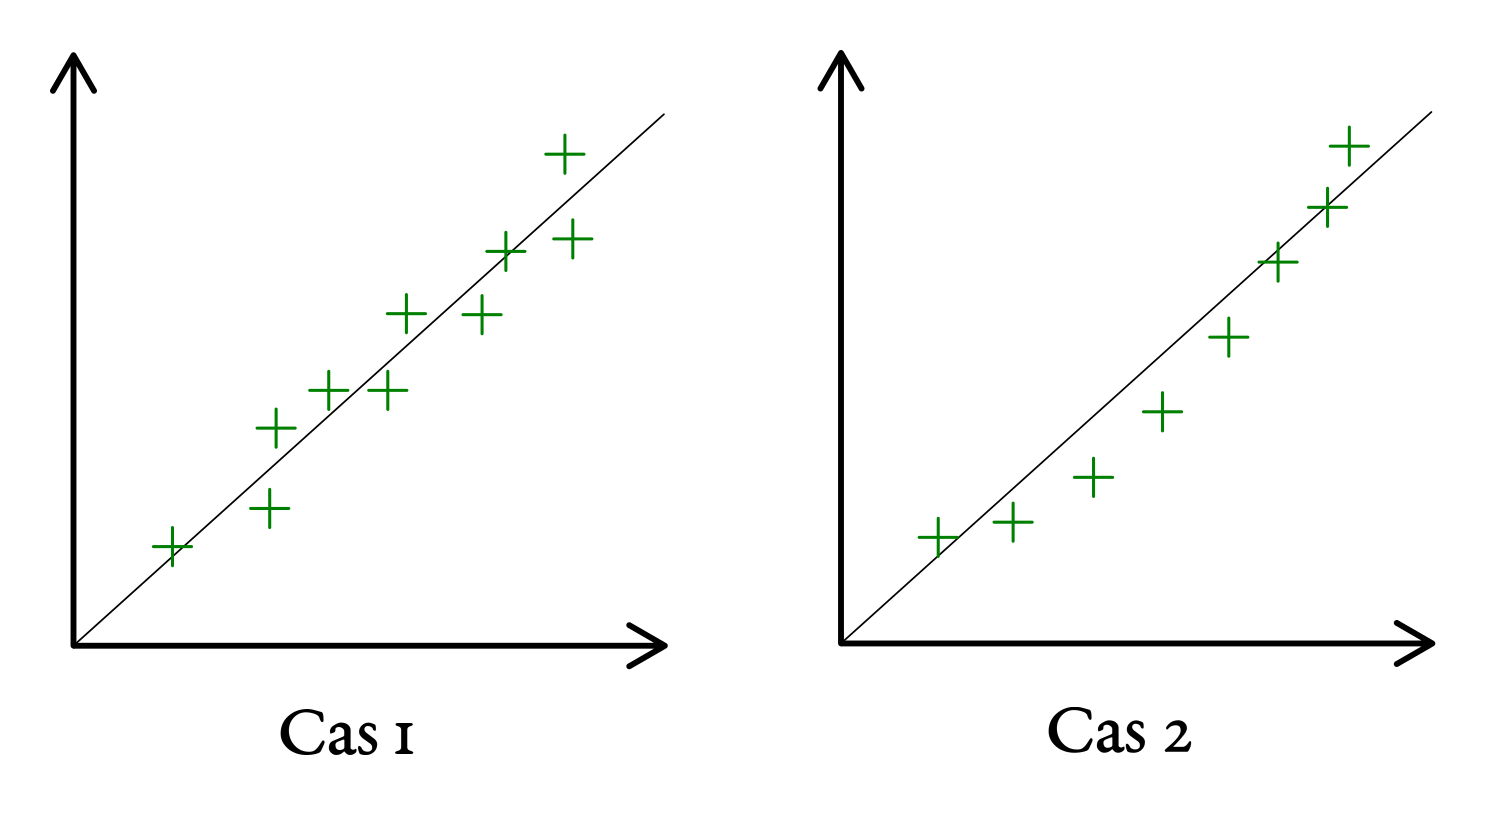
\includegraphics[width=.7\linewidth]{figures/reglin_nl}
	\caption{Exemples de régressions linéaires. Le cas 1 est un modèle validé. Le
		second ne l'est pas.}
	\label{fig:reglin_nl}
\end{figure}

\section{Cas non linéaires}
Dans de nombreux cas, la loi à vérifier n'est ni affine ni linéaire. C'est le
cas de la loi de \textsc{Snell}-\textsc{Descartes} sur la réfraction entre deux
milieux d'indice optique $n_1$ et $n_2$~:
\[
	n_1\sin(i_1) = n_2\sin(i_2)
\]
Avec des mesures de $i_1$ et de $i_2$, il n'est pas possible d'obtenir
directement une droite. Il faut dans ce cas tracer
\[
	y = ax+b
	\qqav
	y = \sin(i_1) \qet x = \sin(i_2)
\]
L'adaptation en \texttt{Python} est relativement directe, mais il faut maîtriser
les opérations sur des listes \textit{via} les calculatrices.
\begin{tcbraster}[raster columns=2, raster equal height=rows]
	\begin{tcb}(expe)<itc>{TI 83+}
		\begin{itemize}[leftmargin=10pt]
			\item Aller sur la case \texttt{L3}, puis \texttt{ENTER}
			\item Entrer la formule (\texttt{L3=sin(L2)} ici), puis \texttt{ENTER}
		\end{itemize}
	\end{tcb}
	\begin{tcb}*(expe)<itc>{Casio 35+}
		\begin{itemize}[leftmargin=10pt]
			\item Dans menu \texttt{RUN}, touche \texttt{OPTN} et \texttt{LIST}
			\item Entrer la formule (\texttt{sin(List2) $\ra$ List3} ici), puis
			      \texttt{EXE}
		\end{itemize}
	\end{tcb}
\end{tcbraster}

\begin{tcb}*(expe)<itc>"wip"{Numworks}
	Travail en cours…
	\vfill
\end{tcb}

\end{document}
